\section{Introducción}\label{sec::intro}
El objetivo de este trabajo es clasificar un conjunto de reseñas de películas mediante análisis de sentimientos, aplicando las técnicas de aprendizaje automático supervisado conocidas como K Vecinos más cercanos y el Análisis de Componentes Principales.

\subsection*{Bag Of Words \& K Vecinos más Cercanos}

K Vecinos Más Cercanos (KNN) es un algoritmo que, dado un conjunto de puntos etiquetados en un espacio real,  permite clasificar otros puntos del espacio de acuerdo a la distancia vectorial entre dicho punto y los puntos de ese conjunto. Para poder usarlo en este problema, se debe encontrar una forma de representar cada reseña como elementos de un espacio que nos permita diferenciar entre reseñas positivas o negativas.\\

Para conseguir este espacio, se identificó al conjunto de palabras usados en todas la reseñas (el vocabulario), y se propuso modelar cada una de ellas como un punto del espacio $R^n$. $n$ es la cantidad de palabras del vocabulario y cada coordenada del punto indica cuanta veces fue usada la $i$-ésima palabra del vocabulario en esa reseña. Al ser interpretadas de esta manera, se espera que el conjunto de puntos generado agrupe espacialmente las reseñas de una misma clase. Es decir, si una reseña es positiva debería encontrarse rodeada por reseñas que, en su mayoría, son positivas.\\

El vocabulario usado por las reseñas consiste en palabras usadas cotidianamente por los usuarios entre las cuales se encuentran preposiciones, nombres, adjetivos, etc. Muchas de estas palabras no modifican la positividad o negatividad de una reseña, por lo que incluirlas al momento de realizar la transformación de los datos pueden generar una mala representación de la relación que estamos estudiando. Además, el espacio generado puede llegar a ser demasiado grande, por lo tanto se busca una forma de optimizar su tamaño descartando las dimensiones (palabras) más y menos frecuentes en la base de datos, ya que, aportan poco y nada de información. Por ejemplo, si eliminamos la preposiciones de una reseña, su positividad o negatividad quedará invariante, y al mismo tiempo se logra reducir el tamaño del sistema y realizar una mejor clasificación de la misma.\\ 

Se puede ver que las palabras más y menos frecuentemente usadas son aquellas que no aportan demasiada información al clasificar reseñas, por lo que las mismas serán eliminadas.

\begin{figure}[H]
\begin{center}
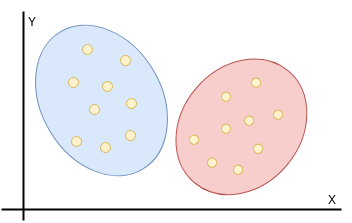
\includegraphics[width=100mm]{img/cjtos.png}
\caption{Representación ideal en $\mathbb{R}^2$ del espacio propuesto.}
\label{intro::esp_vec}    
\end{center}
\end{figure}


El algoritmo de KNN necesita de los siguientes parámetros para armar el modelo inicial:
\begin{itemize}
\item Una base de datos de reseñas etiquetadas, que permitirán al algoritmo clasificar algunos puntos del espacio mencionado.
\item Un entero $k$ que será, dado un punto, la cantidad de vecinos (puntos mas cercanos) evaluados para decidir de que manera se deberá etiquetar al mismo.
\end{itemize}

Una vez obtenido dicho modelo, tomará un nuevo punto, KNN procederá a buscar el subconjunto de los $k$ vecinos más cercanos ya clasificados y lo clasificará según la moda de dicho subconjunto.

\subsection*{Análisis de Componentes Principales}\label{sec::intro::PCA}

El conjunto de vectores formados por las reseñas procesadas puede ser interpretado como una matriz de datos en la que cada fila representa una reseña y, cada columna, una palabra del vocabulario. Esta matriz puede llegar a tener dimensiones exageradamente grandes y, si bien los resultados que se pueden obtener con la misma pueden ser buenos, tambien pueden llegar a ser muy lentos. Se puede ver que hay ciertos elementos del conjunto que son muy parecidos entre si. Eligiendo un representante que caracterice a los grupos más destacados, se puede acelerar el algoritmo de KNN y obtener resultados similares a los que se obtendrían con el modelo original.\\

Esta tarea puede ser lograda aplicando el método de Análisis de Componentes Principales sobre la matriz mencionada. El método, dado un conjunto de vectores en forma de matriz $D$, busca encontrar una transformación lineal  $T$ tal que maximice la varianza entre cada una las componentes de $D$. En \cite{Jolliffe2002Principal} se demuestra que $T$ es la matriz cuyas columnas son los autovectores de la matriz de covarianza de los datos y que los autovalores asociados representan la varianza de cada una de las coordenadas.\\

En otras palabras, se debe centrar los datos en el cero del espacio restando a cada reseña $x_i = (x_{i1},\dots,x_{in})$ su promedio $\mu_i = (x_{i1} + \dots + x_{in})/n$ para poder crear una matriz $X\in\mathbb{R}^{m\times n}$ ($m = $ cantidad de reseñas) en cuyas filas se ubicará al vector $(x_i - \mu)^t / \sqrt{n-1}$ y calcular $M = X^tX$ que queda definida como la matriz de covarianza. \\

Como $M$ es una matriz simétrica semi definida positiva de números reales, se sabe que todos sus autovalores son reales positivos por lo que pueden ser ordenados de tal manera que $|\lambda_1| > |\lambda_2|\geq\dots\geq|\lambda_n|$. Además sus autovectores forman una base de $\mathbb{R}^n$ lo que implica que $M$ es diagonizable. Al tener, $M$, estas propiedades, se puede usar el método de la potencia con deflación para calcular los autovectores asociados a cada $\lambda_i$. \\

El objetivo de esto es reducir la dimensión del espacio a analizar para KNN, por lo que la matriz $T$ que armemos, solo contendrá un subconjunto de los autovectores de $M$. En particular, serán los primeros $\alpha$ ya que estos son los que aseguran mantener las dimensiones de mayor varianza.






% \section{Introducción}

% El presente trabajo práctico propone una introducción a las técnicas de Aprendizaje Automático (Machine Learning) supervisado aplicando conceptos básicos de la materia: autovalores y autovectores, métodos de la potencia,
% descomposición en valores singulares.


% \subsection{El problema a resolver}
% El Análisis de Sentimiento se refiere al conjunto de técnicas de Procesamiento de Lenguaje Natural  (NPL), Ling\"uistica Computacional e Inteligencia Artificial utilizadas para poder extraer, identificar y cuantificar información acerca del estado de ánimo de un sujeto. En particular, nos interesa analizar la polaridad de un texto; es decir, si un texto tiene una emoción "positiva" o "negativa" en lineas generales.
% En este trabajo práctico construiremos un analizador de polaridad para las opiniones sobre películas de usuarios de IMDB.
%  Como muchas aplicaciones prácticas se busca un sistema  que sea flexible en cuanto condiciones de capacidad de procesamiento, memoria y velocidad de una máquina. \\
% Nuestro sistema analizador de polaridad debe clasificar datos de alta dimensión por lo tanto se debe reducir la dimensión, es decir reducción de características principales de una reseña, para permitir una velocidad y consumo de recursos aceptable. 
% Para lograr esto utilizaremos el método de reducción de dimensiones, PCA, junto con el de clasificación kNN. Adicionalmente queremos saber si una reseña cualquiera pertenece a una clase o no.\\
% Se cuenta con una base de datos con $n$ cantidad de reseñas($cant\_res$)tomadas como vectores de tamaño m (el número total de dimensiones de la i-ésima instancia almacenada por filas), etiquetadas por nombres según corresponda. Gracias  a estas etiquetas podemos ir ajustando el modelo de acuerdo al feedback que nos provee la comparación del resultado con la etiqueta. Más adelante en el trabajo se detallan diferentes métricas que se usan para comparar las predicciones que provee el modelo y así estimar un análisis cualitativo del mismo con el fin de ajustar parámetros bajo cierto criterio. \\ 
% Este proceso de aprendizaje y ajuste de parámetros basándose en un conjunto de datos de entrenamiento a los que ya le conocemos la categoría a la que pertenecen cada uno de sus miembros se le denomina aprendizaje supervisado.\\
% El objetivo es utilizar dicha información para, dada una nueva reseña de una clasificación, determinar si pertenece a la base de datos teniendo en cuenta factores de calidad y tiempo de ejecución requeridos.


% \subsection{Método kNN}
% Este algoritmo considera a cada reseña de la base de entrenamiento como un punto en el espacio, para el cual se conoce a qué clase corresponde. Luego, al obtener una nueva reseña, se buscan los $k$ vecinos más cercanos y se le asigna la clase que posea el mayor número de repeticiones dentro de ese subconjunto, es decir, la moda.

% Con este objetivo, representamos a cada reseña de nuestra base de datos como un vector $x_{i} \in R^{m}$ , con
% $1 \leq i \leq n$, $n = \#$ reseñas, e interpretamos las reseñas a clasificar mediante el algoritmo kNN. En otras palabras, nuestra base de datos pasa a ser una matriz $R^{ n \times m}$, donde cada fila es una reseña y la distancia entre reseñas pasa a ser distancia entre vectores.

% Tiene la desventaja de que puede ser muy costoso dependiendo de la dimensión de los objetos y que la clasificación sea lenta dependiendo del contexto. Teniendo en cuenta esto, una alternativa es preprocesar las instancias para reducir la cantidad de dimensiones de las muestras con el objetivo de trabajar con una cantidad de variables más acotada y, al mismo tiempo, buscar que las nuevas variables tengan información representativa para clasificar los objetos de la base de entrada. Utilizaremos uno de estos métodos, Análisis de Componentes Principales(PCA), el cual se detalla a continuación.

% \subsection{Método de Análisis de Componentes Principales(PCA)}

% PCA es un método de extracción de características. El objetivo principal que tiene es reducir la dimensionalidad de un conjunto de observaciones con una gran cantidad de variables, mediante el estudio de la varianzas$-$covarianzas entre las variables que integran los datos de entrada.\\
% A partir de la proyección de los datos de entrada sobre las direcciones de máxima varianza se obtendrá un nuevo espacio de representación de los datos en el que se puede eliminar fácilmente aquellas componentes con menor varianza, garantizando la mínima pérdida de información. Sin embargo, este método puede  presentar algunas desventajas como la dificultad de análisis de los datos resultantes o una función de coste poco robusta frente al ruido. Se verá experimentalmente cuando podría ser adecuado su uso.














